\chapter{Bilder}
How to display pictures:

\begin{figure}[H] %%[H] for "here" so that the picture is not moved to the end of the paragraph
  \centering %% picture is centered
  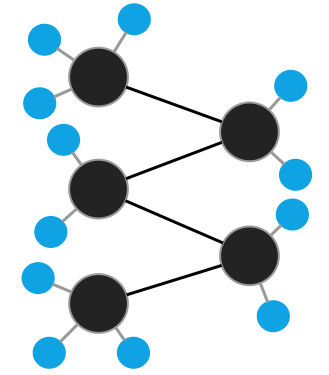
\includegraphics[width=.25\textwidth]{graphics/molecule}
  \caption[Caption for the list of figures]{Caption display below the picture}
  \label{fig:pic1} %% label to reference the picture within the text
\end{figure}
\noindent
Figure \ref{fig:pic1} and \ref{fig:pic2} use the same file. With the command \verb+width=y.x\textwith+ the size can be adjusted.
\begin{figure}[H] %%[H] for "here" so that the picture is not moved to the end of the paragraph
  \centering %% picture is centered
  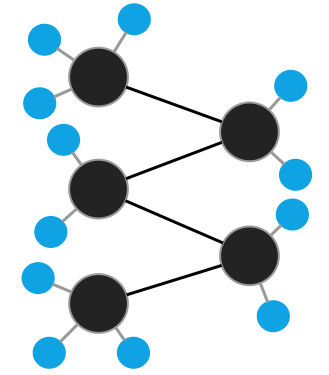
\includegraphics[width=.5\textwidth]{graphics/molecule}
  \caption[Caption for the list of figures]{Caption display below the picture}
  \label{fig:pic2} %% label to reference the picture within the text
\end{figure}
\noindent
\section{Multiple Pictures}
Multiple figures (see Figures \ref{fig:subfig1} and \ref{fig:subfig2} or in general Figure \ref{fig:subfigs}):
\begin{figure}[H]
  \centering
  \subfloat[Subcaption for the first graphic]{
  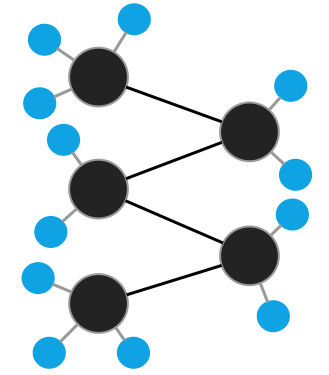
\includegraphics[width=.5\textwidth]{graphics/molecule}
  \label{fig:subfig1}
  }
  \subfloat[Subcaption for the second graphic]{
  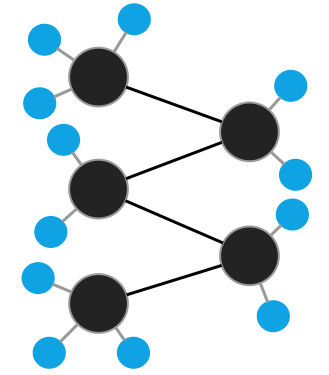
\includegraphics[width=.5\textwidth]{graphics/molecule}
  \label{fig:subfig2}
  }
  \caption[Caption for multiple graphics in the list of figures]{(\ref{fig:subfig1}) Some text for the first graphic. (\ref{fig:subfig2}) Some text for the second graphic.}
  \label{fig:subfigs}
\end{figure}
\noindent